\documentclass{jsarticle}
\usepackage[dvipdfmx]{graphicx}
\usepackage{listings}
\usepackage{afterpage}
\begin{document}
\title{課題8 ラベリング}
\author{13EC060 武澤 裕介}
\maketitle
\begin{abstract}
matlabを用いて、2値化を行った後、ラベリングを行い考察する。
\end{abstract}
\section{ラベリング}
まず、今回使用する原画像を図1に示す。


\begin{figure}[htbp]
 \begin{center}
  
\includegraphics[width=5cm,height=5cm]{index.jpg}
 \end{center}
 \caption{原画像}
\end{figure}

\begin{lstlisting}[basicstyle=\ttfamily\footnotesize, frame=single]
filename = uigetfile('*');
ORG=imread(filename); % 原画像の入力
ORG = rgb2gray(ORG); colormap(gray); colorbar;
imagesc(ORG); axis image; % 画像の表示
pause; % 一時停止
 \end{lstlisting}
を用いてまず入力画像のグレースケール画像を表示させる。

\newpage
\begin{figure}[htbp]
 \begin{center}
  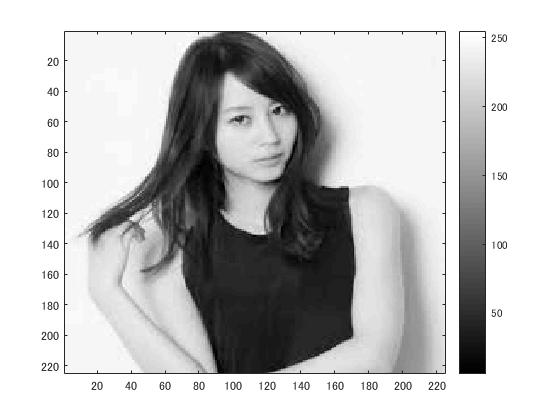
\includegraphics[width=10cm]{8-0.jpg}
 \end{center}
 \caption{グレースケール画像}
\end{figure}

次に
\begin{lstlisting}[basicstyle=\ttfamily\footnotesize, frame=single]
IMG = ORG > 128; % 閾値128で二値化
imagesc(IMG); colormap(gray); colorbar; % 画像の表示
pause;
 \end{lstlisting}
を用いて画像を二値化し表示する。

\newpage
\begin{figure}[htbp]
 \begin{center}
  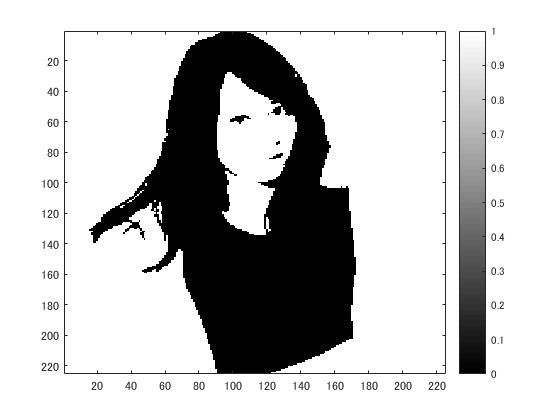
\includegraphics[width=10cm]{8-1.jpg}
 \end{center}
 \caption{二値化画像}
\end{figure}

最後に
\begin{lstlisting}[basicstyle=\ttfamily\footnotesize, frame=single]
IMG = bwlabeln(IMG);
imagesc(IMG); colormap(jet); colorbar; % 画像の表示
pause;
 \end{lstlisting}
を連結成分のラベリングを行い、表示する。

\newpage
\begin{figure}[htbp]
 \begin{center}
  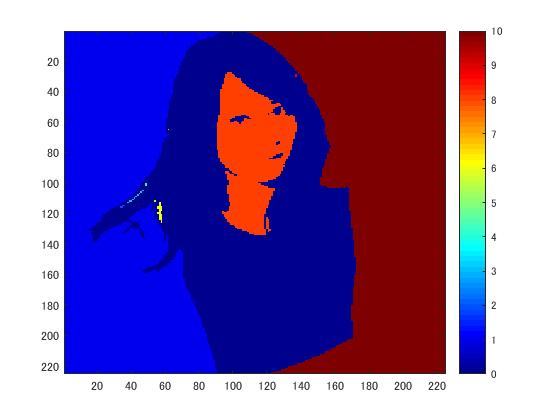
\includegraphics[width=10cm]{8-2.jpg}
 \end{center}
 \caption{ラベリング}
\end{figure}


\section{考察}
今回ラベリング行った、図3と図4を比較すると連結された領域どうしは、色が変わってない事が分かる。

\end{document}